\chapter{Working Week}
Working Week for Venturer camp was scheduled to begin on Wednesday 2 August, and run until midday on Saturday 5 August, when we allowed campers onto the site. During On-Site pre-Camp, the Camp Coordinator and Working Week coordinator decided that they would arrive on site on Sunday 30 July. \\

For the duration of Working Week and Pre Working Week, we were camping \& eating with Lewisham \& Greenwich, who were having their district summer camp on Pitches 6 \& 7. This was hugely beneficial to the Venturer Camp team as we were able to be fed and have shelter, without having to deal with it ourselves. However, from a KP's perspective: the Venturer Camp team was a nightmare to cater for. The KP has recommended not to do it in this way again, and that a separate KP should be sought for Working Week due to conflicting requirements of District Camp and Working Week. Members of the Working Week team were strongly encouraged to get involved with the meal preparation and clean up, to aid the Lewisham \& Greenwich team. The KP gave us a requirement of numbers for each meal, then it was up to the Venturer Camp team to find the people to fill this.\\

Having Lewisham \& Greenwich on site for the duration of Working Week also meant that we had access to the Luton Van which they had hired to transport their equipment. This proved extremely valuable as we were able to move equipment around the site with ease. It's helpful to have a few people confident to drive the van on-site as the requirement of this being on one or two people makes it more of a complex operation to move the van with needing to have the right people in the right places. \\

The pre Working Week days were used to organise and extricate equipment from the Bunkhouse storage rooms. It was decided that these days were needed after reviewing the relatively unorganised mound of equipment during on-site pre-camp. These days were instrumental in the success of Working Week, as there wasn't lots of time wasted on the first official day pulling tent poles out of a tiny room where only a few people could fit at once.\\

\begin{figure}[ht]
    \centering
    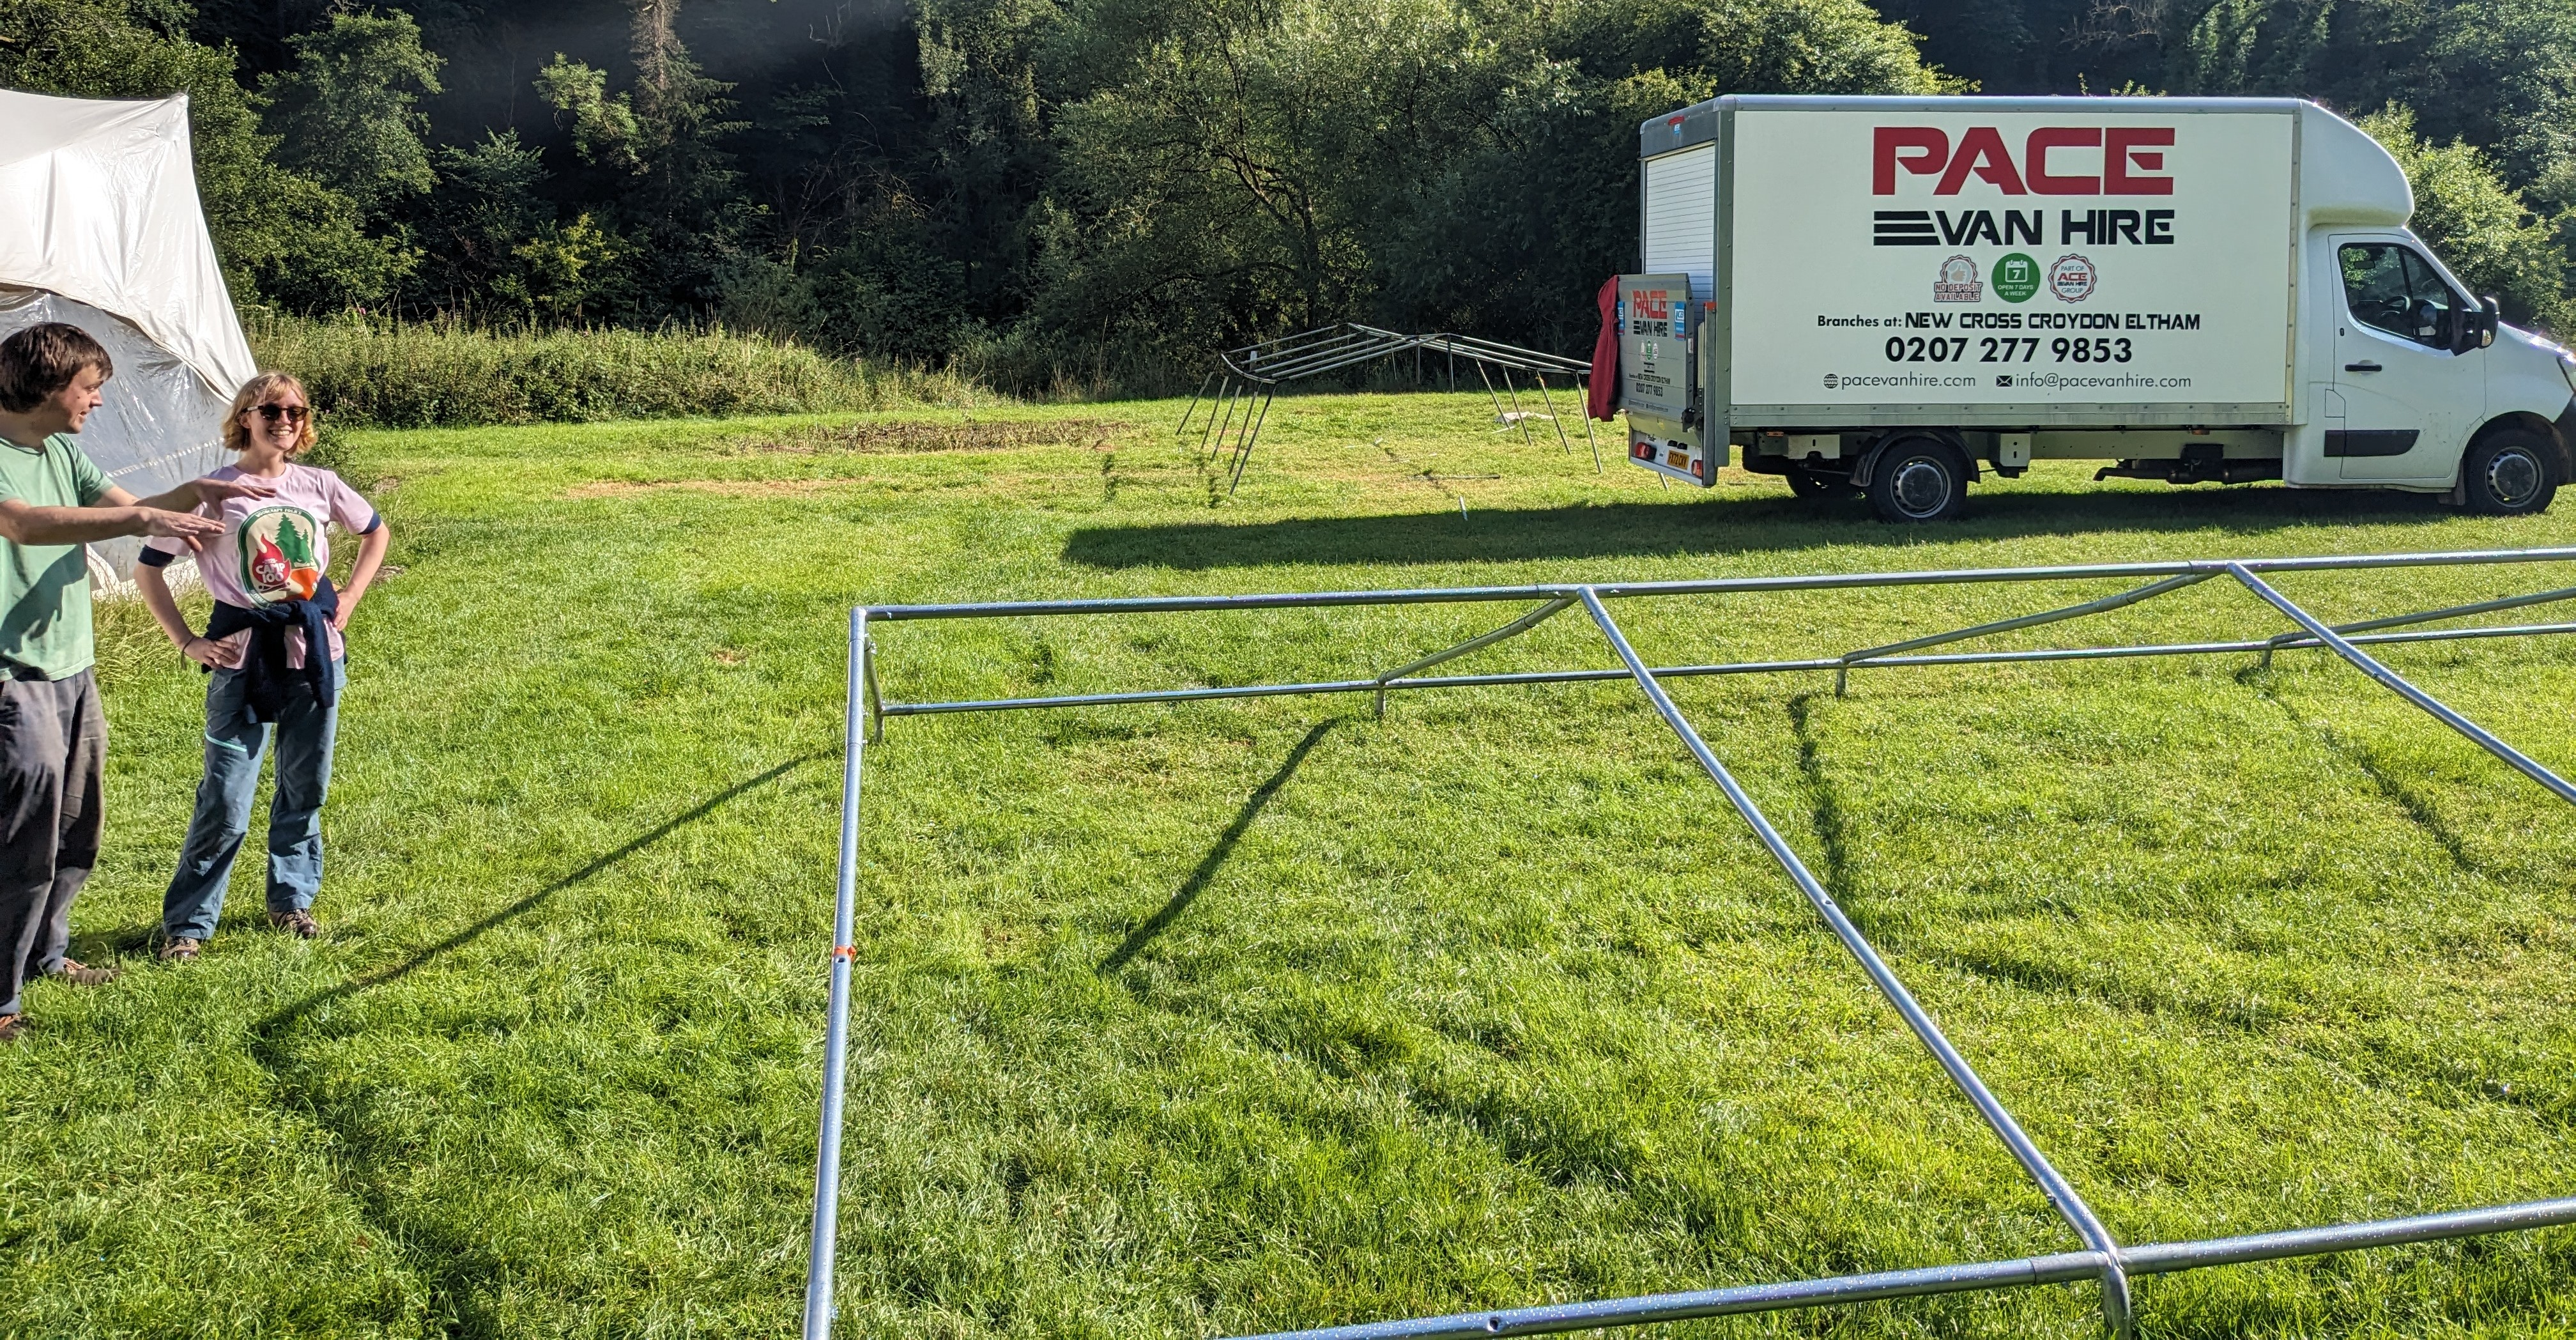
\includegraphics[width=0.8\textwidth]{assets/c100-coords-survey-5x10m-marquee.jpg}
    \caption{Camp100 coordinators survey one of the surviving 5x10m marquees as it's put up (\textit{TB})}
\end{figure}

On Tuesday 1 August, the Concordia team arrived to site. They spent the afternoon getting to know each other and the site with the ESC volunteers; then from morning on Wednesday 2 August - they got stuck in with the Working Week tasks. Altogether, we had 42 people book for some of Working Week, with 27 of these being on site from 2 August. This felt like the right number, however some additional people will always be useful! We managed to get all the required tasks done, however some of the administration was a bit of a squeeze towards the end. \\

As more people arrived for Working Week, they were keen to camp where they would be for the duration of the camp, rather than pitching on Pitch 6 for two nights then having to move. It was agreed that where no further groups were scheduled to be on the pitches, then Working Week attendees could camp where their village would be, this worked fine for the most part. \\

Having a dedicated coordinator for Working Week is extremely important. This is someone who works closely with the Coordinator to understand exactly what tasks need to be done and can lead the operational aspect of getting the site configured - leaving the Coordinator to deal with other, more complex problems. We were fortunate, in that there weren't many other problems - leaving the Coordinator to support with the site setup. A vague plan was devised ahead of time, building on discussions had at on-site pre-camp. This was useful and allowed for the Coordinator \& Working Week Coordinator to allocate tasks, especially surrounding people setting up their spaces on camp.\\

Each morning, a daily briefing was held over Breakfast - which enabled tasks for the day to be divided up \& people to share where they might need additional support throughout the day, or plan use of resources such as the van. Throughout the day, the Coordinator and Working Week Coordinator kept up to date with different teams - ensuring everyone was able to get on with their tasks. Walkie Talkies were used for communication, which is vital. It's imperative that these arrive to site fully charged and ready to go as waiting around for them to be charged wastes time.\\

\begin{figure}[ht]
    \centering
    \includegraphics[width=0.8\textwidth]{assets/working-week-breifing.jpg}
    \caption{Working Week Crew (\textit{TB})}
\end{figure}

Generally speaking, the right people were on site for Working Week. It would have been useful to have some more representatives from each centre present to ensure they were set up how they wanted it to be, however the Programme coordinator was able to fill in this gap. It proved very helpful to have a number of people who were able to support the large tasks, such as the Solar Array installation where a few key individuals were the masterminds behind it. Having additional people enabled the masterminds to conduct rather than do - preserving their energy for the camp itself!\\

During the week, large pieces of infrastructure got delivered to site. Much of this had been arranged by one person, with only them knowing the details of it or these details being stashed in a Google Drive folder somewhere. It would be useful for future events, for this information to be collated into the Working Week timetable so that we are able to easily allocate where the Porta-Loos are being placed or work out how big of a space we need to leave for the Main Marquee!\\

During the week, the Coordination \& Event Administration team worked closely with the Biblins site staff, forming relationships which proved extremely valuable for the camp.\\

Towards the end of the week, there were still a number of large groups on site who were scheduled to leave early on 5 August, the first day of camp. It would be beneficial to ensure that the site is booked for at least one day either side of the event itself as having the groups around made some things more complex, such as access to pitches. Generally speaking, other than one incident, the groups who were present on site during Pre Working Week \& Working Week itself were fine with us and didn't mind us being there. The incident was in relation to a group camping at the Eastern end of the site not wanting people driving past their pitch to access the canoe turning circle, which was required to turn the van around. 
